\documentclass[a4paper,11pt]{article}
\usepackage[utf8x]{inputenc}
\usepackage[T1]{fontenc}
\usepackage{fullpage}
\linespread{1.1}
\usepackage{mathpazo}
\usepackage{listings}
\lstset{
%language=TeX,
breaklines=True}
\usepackage[]{color}
\usepackage[version=3]{mhchem}
\usepackage{float}

\usepackage[pdftex]{graphicx}
\graphicspath{{./figs/}}
\usepackage[update,verbose=false]{epstopdf}

\usepackage[]{hyperref}

% New commands which ease the work. Units and relative uncertainties
\newcommand{\unit}[1]{\ensuremath{\, \mathrm{#1}}}
\newcommand{\relerr}[1]{\ensuremath{ \cfrac{\Delta #1}{#1}}}
\newcommand{\eten}[1]{\ensuremath{ \times 10^{#1}}}
\newcommand{\DP}[2]{\ensuremath{\cfrac{\partial #1}{\partial #2}}}
\newcommand{\DD}[2]{\ensuremath{\cfrac{\mathrm{d} #1}{\mathrm{d} #2}}}
\newcommand{\dd}[1]{\ensuremath{\mathrm{d}#1}}

\title{Getting good quality graphics inside a \LaTeX\ document}
\author{Ignas Anikevicius}

\begin{document}

\maketitle

\section{Introduction}

For publications and scientific articles, reports and thesis the most important
thing is to make well looking graphics. For that there are several guidelines,
which help one to get his figures look professionally, but at the same time not
to overdo things as there is a limit of how good the quality has to be.

\begin{enumerate}
    \item Use vector graphics as much as possible. Especially where there is a
        lot of text in the figure. But remember, if you 'convert' a jpg to eps
        or svg or any other vector graphics format, you will \textbf{not} gain
        any quality. More on this, please use
        \href{http://www.google.co.uk}{Google}
    \item If you have to use raster graphics, please select \verb|png| format as
        a better alternative where possible
    \item If you use raster graphics, do not exceed the final resolution of the
        picture to more than 600dpi as most of the printers are printing at
        300dpi or 600dpi, so anything more than that might just be wasted time
        while waiting the figure to be rendered. Of course if you have a good
        reason why you need more than 600dpi, then go ahead.
    \item Have a high quality copy of your figure somewhere in your computer.
        This is because while converting from one format to another one can
        \textbf{not} improve the quality.
\end{enumerate}

If you feel that you have not found enough information on the graphics usage in
\LaTeX, please refer to these websites:
\begin{itemize}
    \item
        \href{https://secure.wikimedia.org/wikibooks/en/wiki/LaTeX/Floats,_Figures_and_Captions}{Floats,
        Figures and Captions}
    \item
        \href{https://secure.wikimedia.org/wikibooks/en/wiki/LaTeX/Importing_Graphics}{Importing
        Graphics}
    \item
        \href{https://secure.wikimedia.org/wikibooks/en/wiki/LaTeX/Creating_Graphics}{Creating
        Graphics}
\end{itemize}

\section{Inserting a simple figure}

Inserting a simple figure can be as easy as:
\lstinputlisting{fig1.tex}
which will produce the following:
\begin{figure}[H]
    \begin{center}
        \includegraphics{plot3.eps}
    \end{center}
    \caption{First plot}
    \label{fig:figure1}
\end{figure}


However one can immediately notice, that the figure is not scaled and the
caption text is slightly to far from the actual figure, so these small changes
will fix these nuances:
\lstinputlisting{fig2.tex}
And our figure will look as follows:
\begin{figure}[H]
    \centering
    \setlength{\unitlength}{\textwidth}
    \vspace{-5mm}
    \begin{picture}(1,.75)
        \put(0,0){\includegraphics[width=.4\unitlength]{plot1.eps}}%
        \put(0.1,0.6){$f(x) = \cfrac{\sin{x}}{x}$}
        \put(0.14,0.40){$f(x) = e^{-x^2}$}
        \put(0.14,0.40){$f^2(x)$}
    \end{picture}%
    \vspace{-10mm}
    \caption{Overlaying \LaTeX\ commands on top of the figure.}
    \label{fig:plot2}
\end{figure}


\section{Directory setting for graphics, their formats and \LaTeX\ compilers}

The most convenient way nowadays to produce documents from \LaTeX\ source code
is to use the \verb|pdftex| or \verb|pdflatex| compiler. It is very convenient
as one does not need to convert the \verb|.ps| file every time before viewing it
with a viewer. Also there are other benefits to use this compiler.

Using \verb|graphicx| package with this compiler lets you use \verb|.jpg|,
\verb|.png| and \verb|.pdf| graphics inside your document. You might ask:
``What about my \verb|.eps| figures?'' The simple answer is to use
\verb|epstopdf| package, which would convert \verb|.eps| figures to \verb|.pdf|
figures on-the-fly.

What is more, which \verb|graphicx| package it is possible to give directory
names where \LaTeX\ should search for figures. The best example would be the
preamble of this file:
\begin{lstlisting}
\usepackage[pdftex]{graphicx}
\graphicspath{{./figs/}}
\usepackage[update,verbose=false]{epstopdf}
\end{lstlisting}

This means, that the \verb|epstopdf| package will convert the \verb|.eps|
graphics only when they are newer than the \verb|.pdf| versions, which might
speed up the compiling time significantly.

\section{Overlaying a figure with \LaTeX\ code}

This is the most interesting capability of \LaTeX\ although it might be
considered as 'fiddly' by some users, as it requires some trial and error, but
it can be very useful in some cases (eg. Having a lot of figures with chemical
structures and getting them cross-referenced and numbered correctly).

\end{document}

% Editor configuration:
% vim: tw=80:spell:spelllang=en_gb
